
\documentclass[aspectratio=169,xcolor=dvipsnames]{beamer}
\usetheme{SimpleDarkBlue}

\usepackage{hyperref}
\usepackage{graphicx} 
\usepackage{booktabs} 


\title{An Insight into Edge and Fog Computing}

\author{Can Tian - Dilyara Daroglu}

\institute
{
    Wissenschaftl. Arbeitstechniken u. Präsentation \\
    Paris Lodron University of Salzburg 
}
\date{}



\begin{document}

\begin{frame}
    \titlepage
\end{frame}

\begin{frame}{Overview}
    \tableofcontents
\end{frame}

\section{INTRODUCTION}

\begin{frame}{TRADITIONAL DATA PROCESSING STEPS}
    \begin{itemize}
        \item \textbf{Data Collection:} Data collecting devices (sensors, cameras, IoT
devices)
        \item \textbf{Data Transmission:} Data to Central Server or Cloud Data Center
        \item \textbf{Data Processing}
        \item \textbf{Response Transmission:} Processing Result to Original Device
        \item \textbf{Action Execution}
    \end{itemize}
\end{frame}


\section{DEFINITIONS}

\begin{frame}{EDGE COMPUTING}
    \begin{itemize}
        \item \textbf{Nearby Processing – at the
"Edge" of the Network}
        \begin{itemize}
            \item Local Systems
            \item IoT devices themselves (sensors,
            cameras, gateways etc.)
        \end{itemize}
    \end{itemize}
\end{frame}
\begin{frame}{EDGE COMPUTING...}
    \begin{itemize}
        \item reduces time and effort.
        \item saves bandwidth, saves cost.
        \item can work with limited or no internet connectivity.
        \item eliminates delay and congestion.
    \end{itemize}
\end{frame}

\begin{frame}{EDGE COMPUTING}
    \begin{figure}
    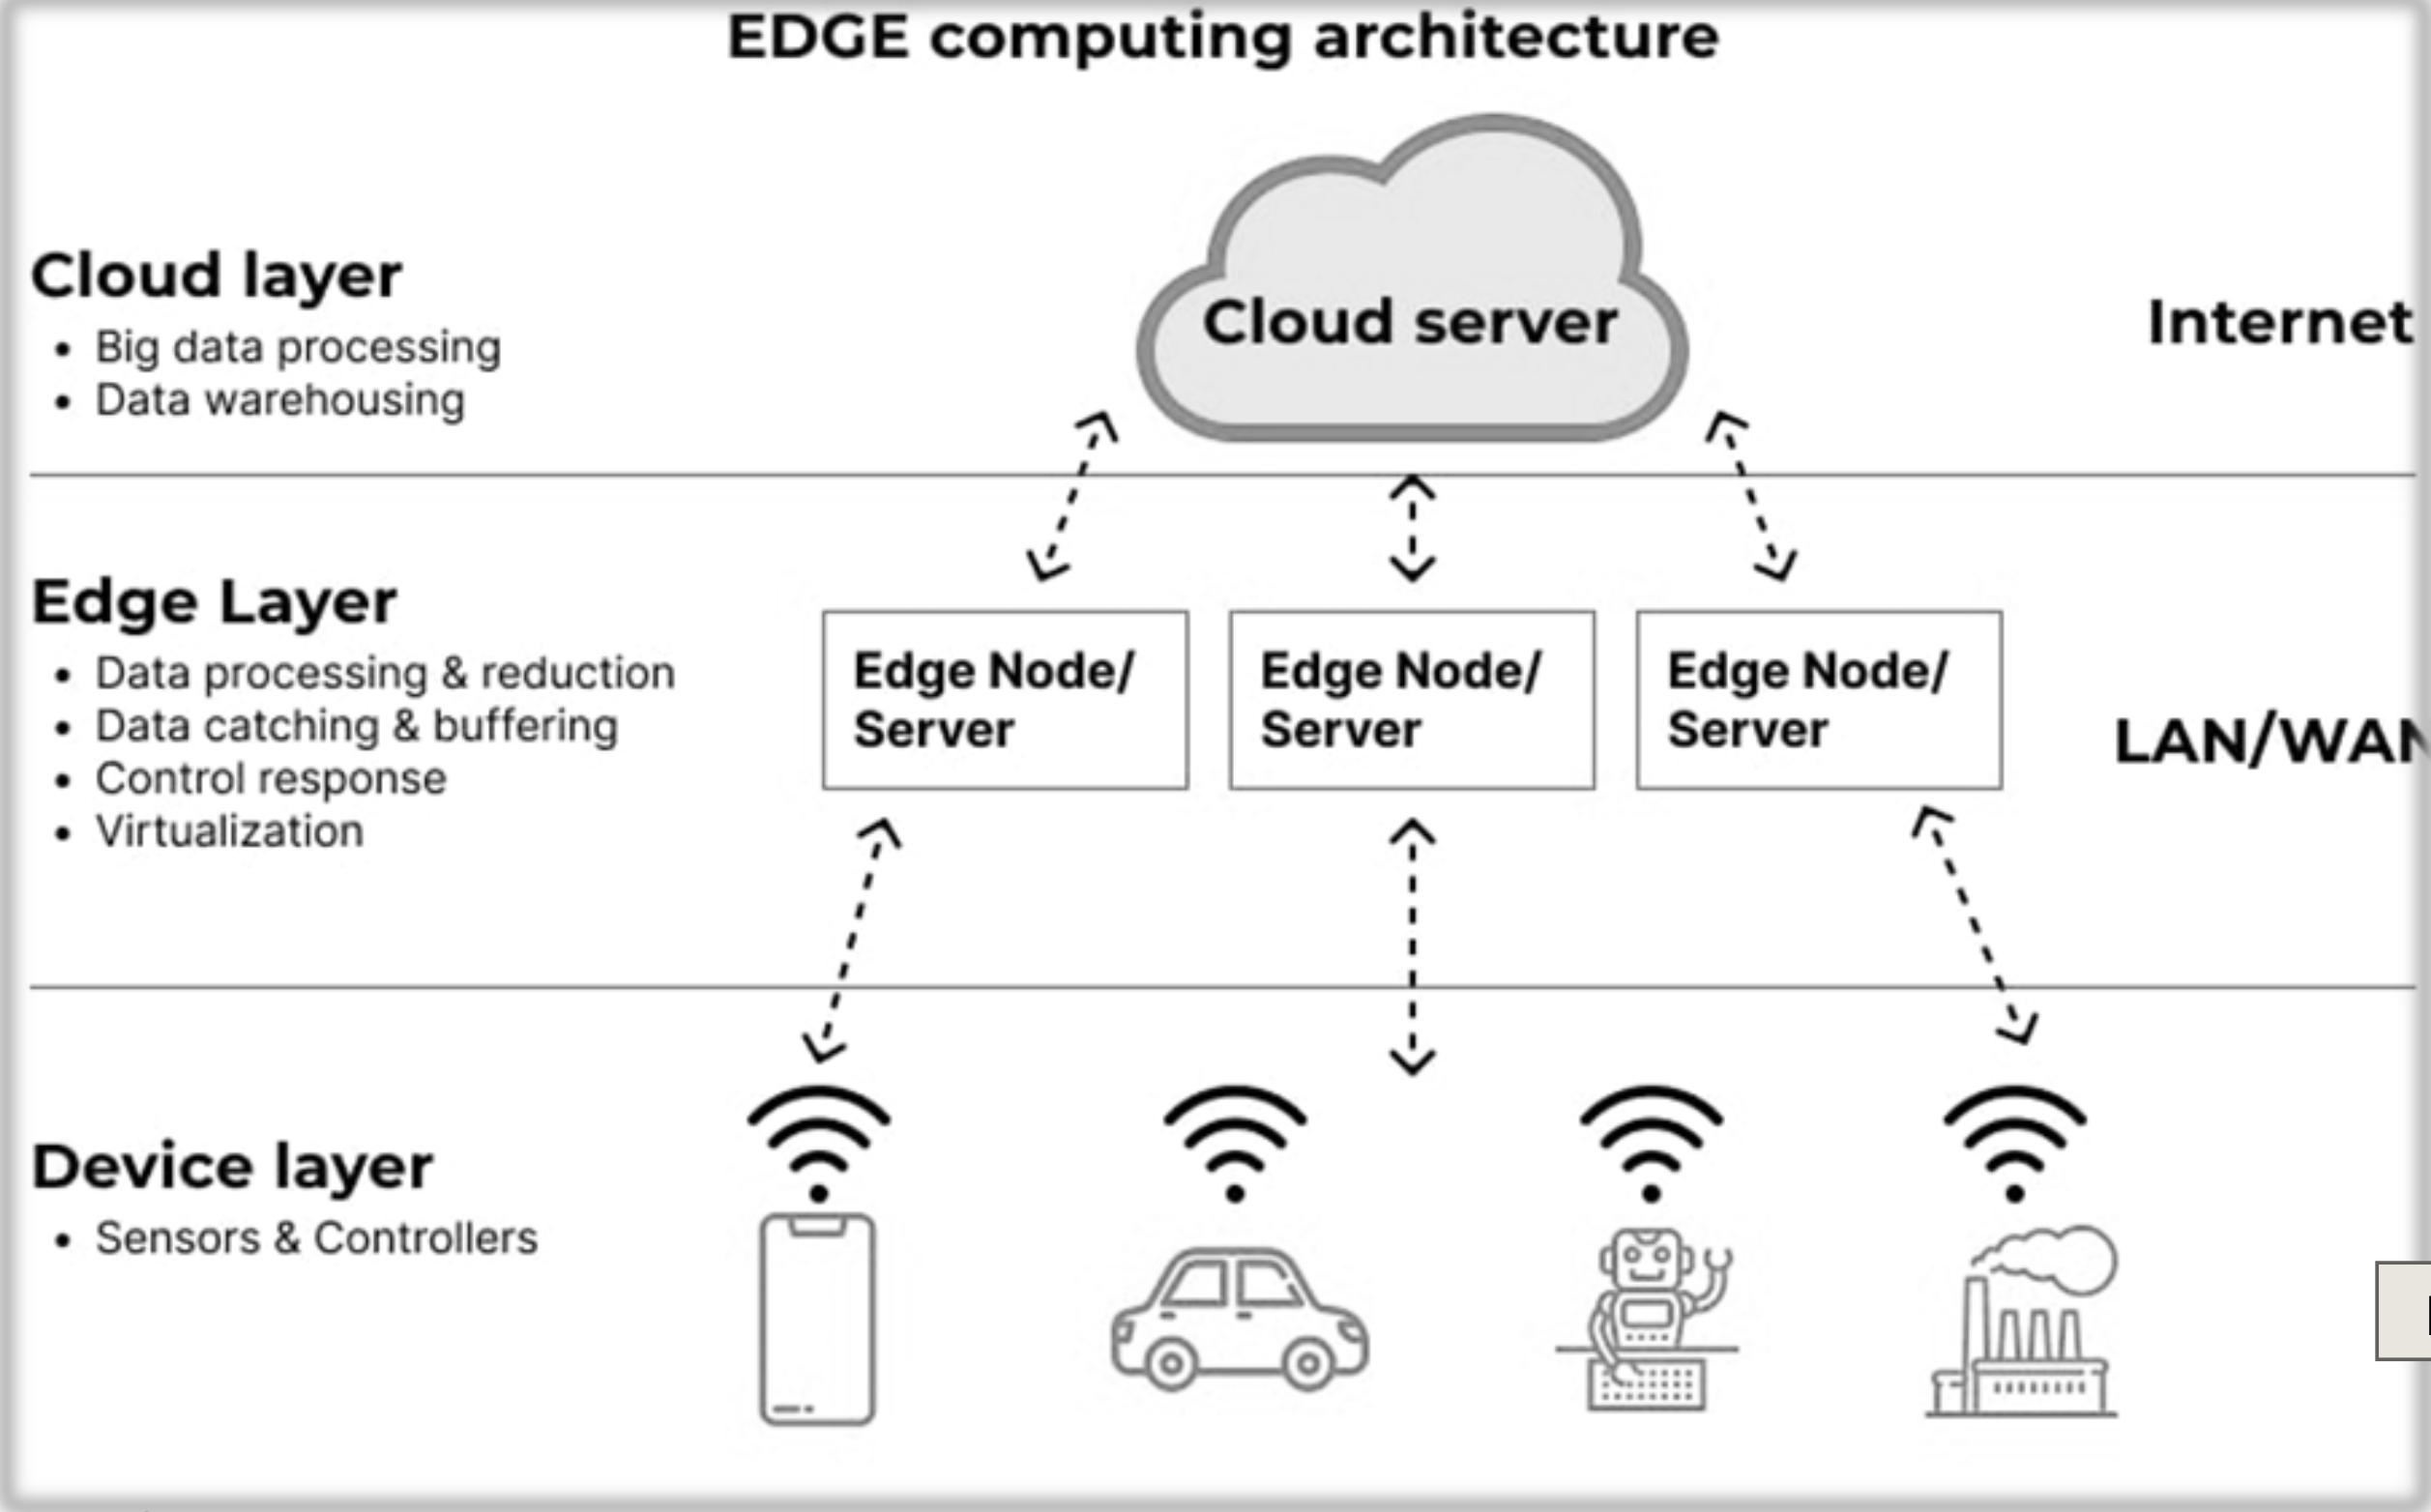
\includegraphics[width=0.6\linewidth]{edge.png}
    \caption{[1] }
    \end{figure}
\end{frame}
\begin{frame}{EXAMPLE - SELF DRIVING CAR}
    \begin{figure}
    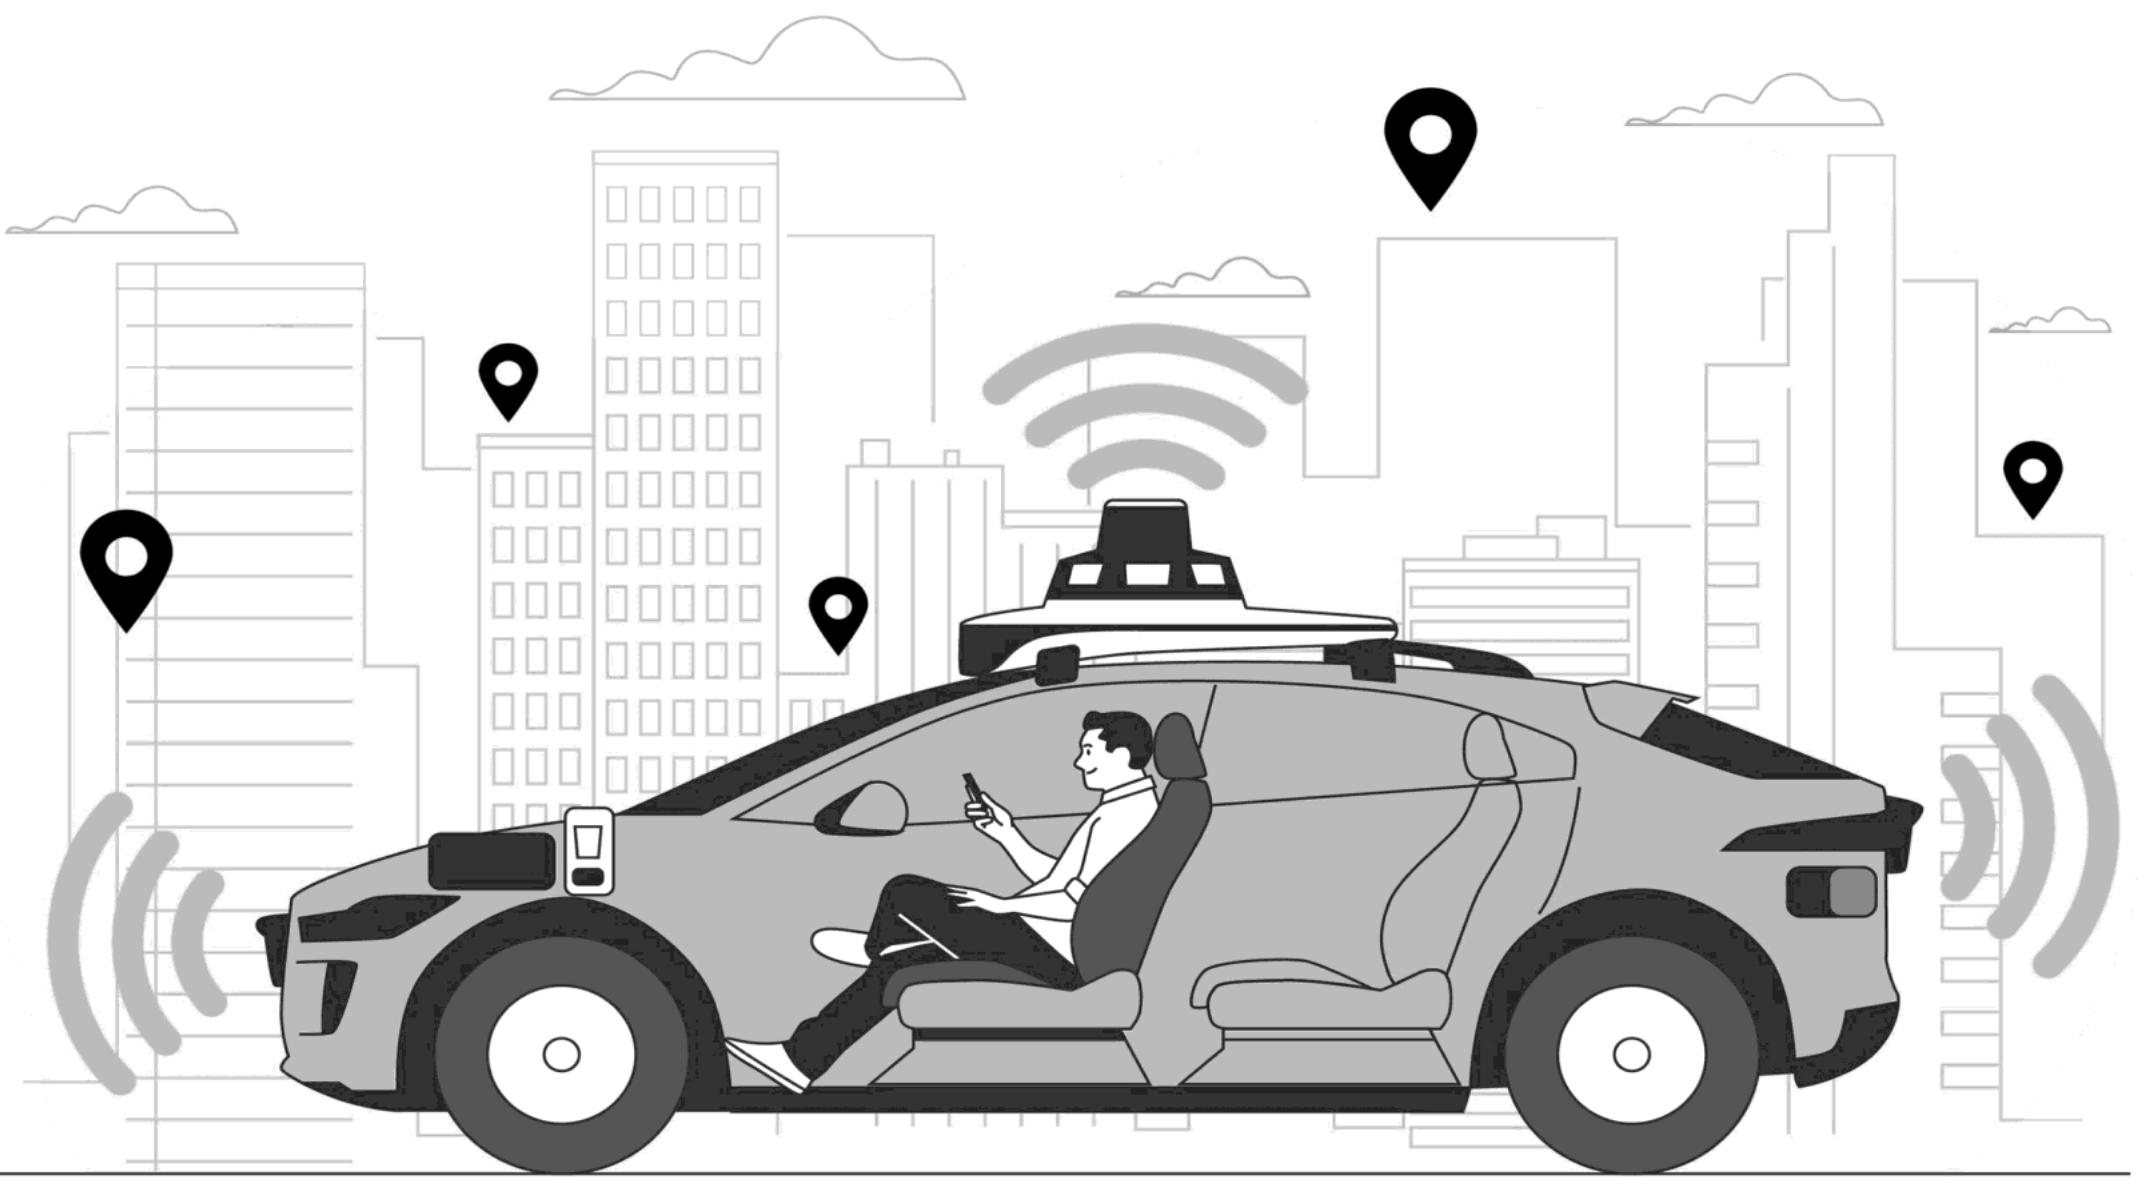
\includegraphics[width=0.7\linewidth]{carexample.png}
    \caption{[2]}
    \end{figure}
\end{frame}
\begin{frame}{Table}
    \begin{table}
        \begin{tabular}{l l l}
            \toprule
            \textbf{Feature} & \textbf{Without Edge Computing } & \textbf{With Edge Computing} \\
            \midrule
            Data Processing         & Distant Cloud           & Local               \\
            Latency         & High           & Low               \\
            Bandwidth Use         & High           & Low               \\
            Internet Dependence         & High           & Low               \\
            \bottomrule
        \end{tabular}
        \caption{DATA PROCESSING COMPARISON}
    \end{table}
\end{frame}
\begin{frame}{GRAPH}
    \begin{figure}
    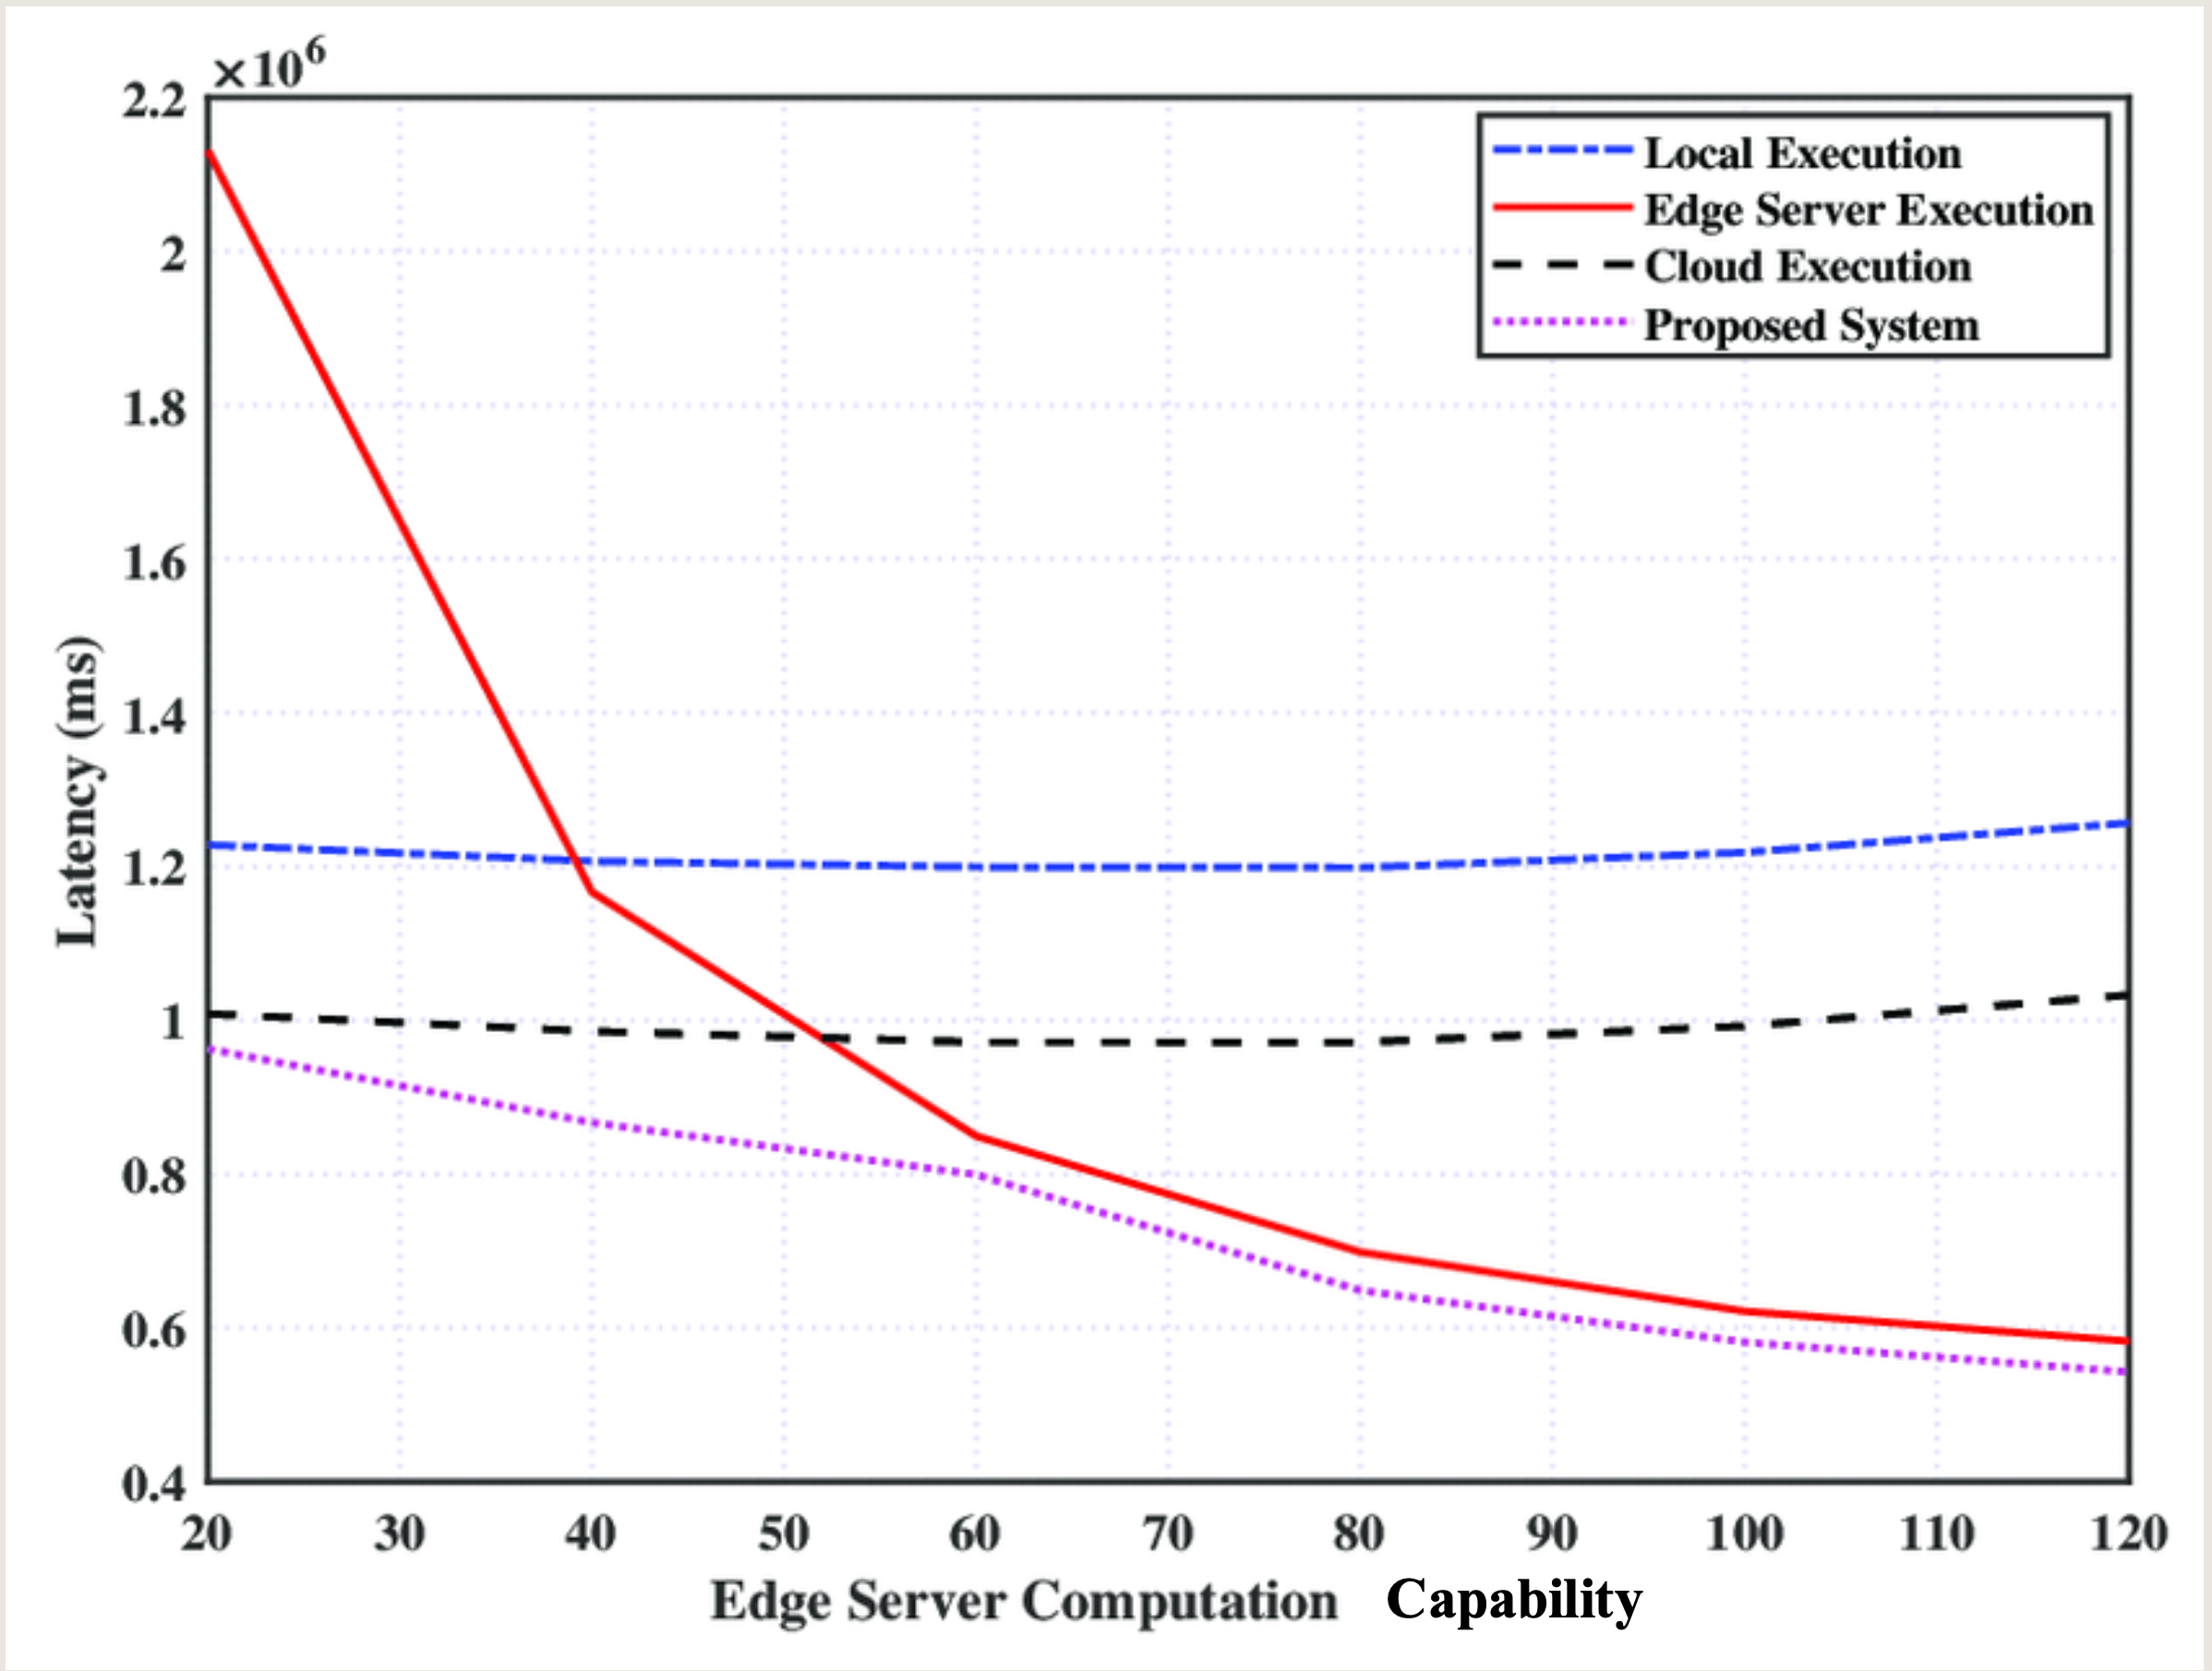
\includegraphics[width=0.56\linewidth]{graphicservercomputation.png}
    \caption{[3]}
    \end{figure}
\end{frame}
\begin{frame}{FOG COMPUTING}
    \begin{itemize}
        \item \textbf{Fog Nodes - Processing in the Middle}
        \begin{itemize}
            \item Local Systems
            \item Local Devices
        \end{itemize}
    \end{itemize}
\end{frame}

\begin{frame}{FOG COMPUTING...}
    \begin{itemize}
        \item reduces load on edge devices.
        \item provides a nearby helper to edge devices.
        \item makes large-scale systems more efficient.
        \item reduces latency, bandwidth use and de-centers load.
    \end{itemize}
\end{frame}

\begin{frame}{FOG COMPUTING}
    \begin{figure}
    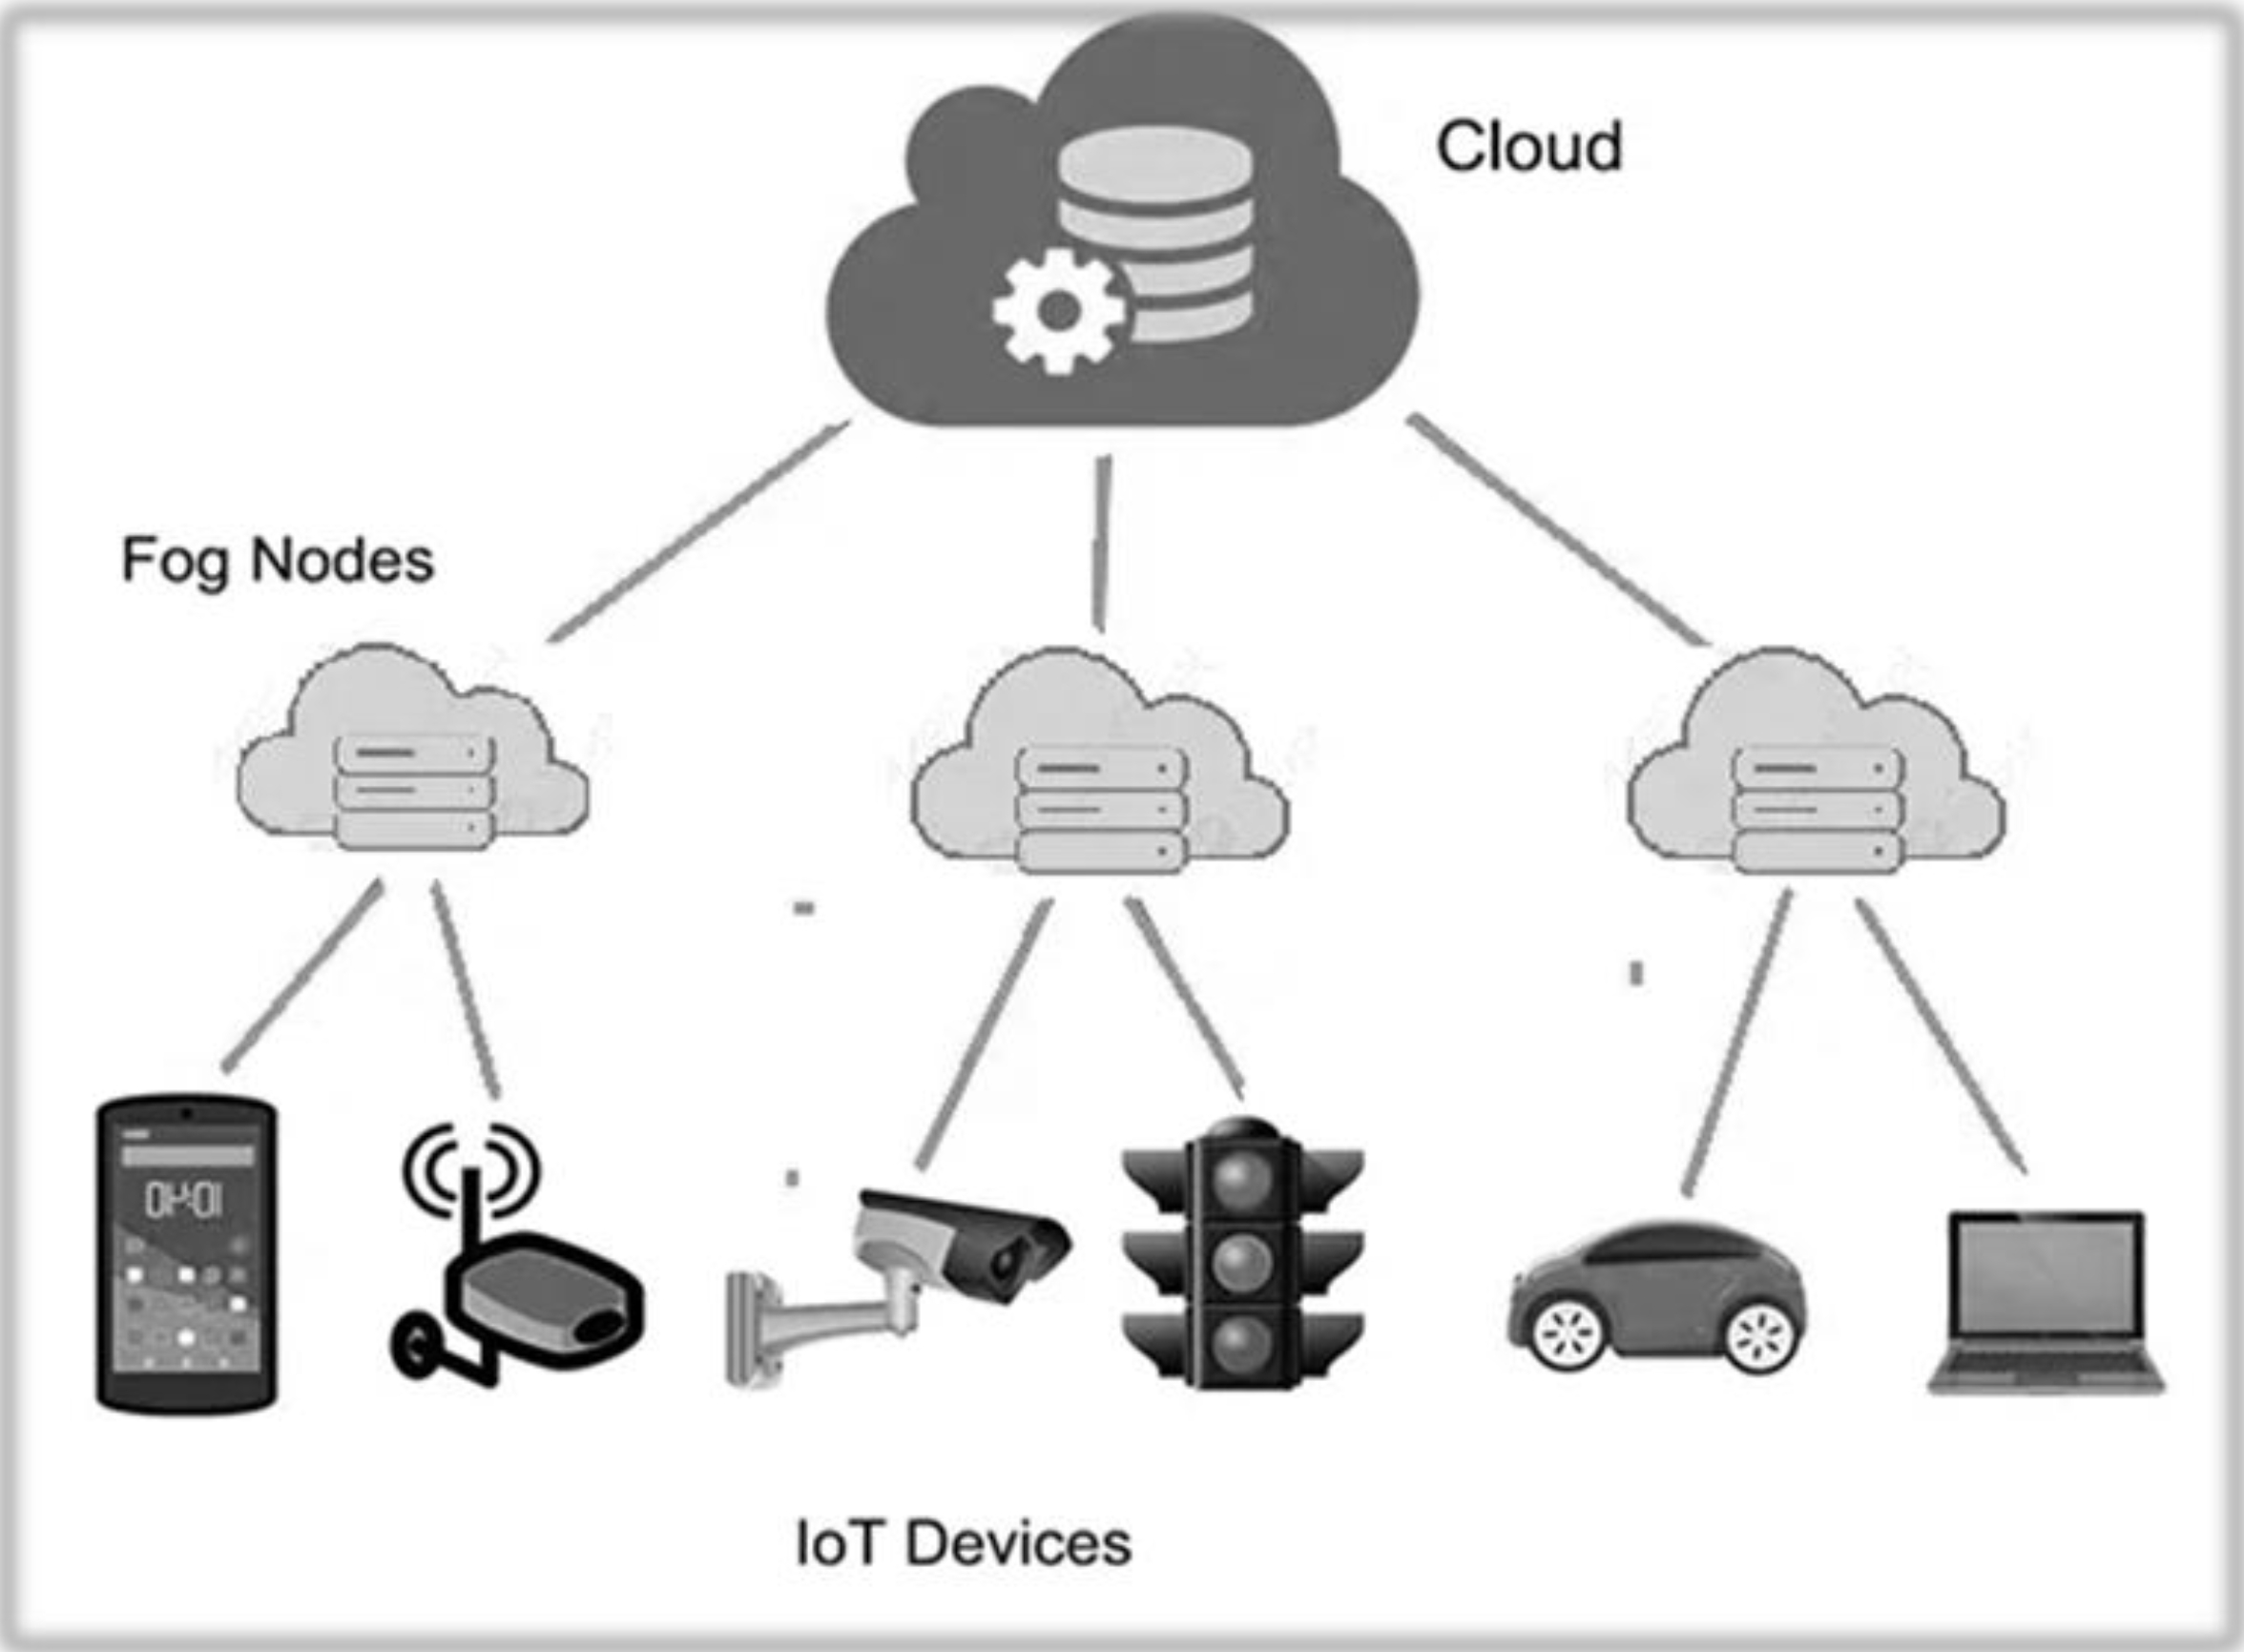
\includegraphics[width=0.57\linewidth]{fogcomputing.png}
    \caption{[4]}
    \end{figure}
\end{frame}

\begin{frame}{Table}
    \begin{table}
        \begin{tabular}{l l l}
            \toprule
            \textbf{Feature} & \textbf{Without Fog Computing } & \textbf{With Fog Computing} \\
            \midrule
            Data Processing         & Distant Cloud           & Distributed locally               \\
            Latency         & High           & Low               \\
            Bandwidth Use         & High           & Low               \\
            Scalability         & Limited           & Improved               \\
            \bottomrule
        \end{tabular}
        \caption{DATA PROCESSING COMPARISON}
    \end{table}
\end{frame}

\begin{frame}{Table}
    \begin{table}
        \begin{tabular}{l l l}
            \toprule
            \textbf{Feature} & \textbf{Edge Computing } & \textbf{Fog Computing} \\
            \midrule
            Data Processing         & At the device, or close           & Local nodes near the edge               \\
            Use case example         & Real-time actions           & Larger-scale systems               \\
            Latency        & Extremely low           & Low               \\
            Power         & Device Dependent           & Helper nearby systems               \\
            \bottomrule
        \end{tabular}
        \caption{FOG AND EDGE COMPUTING COMPARISON}
    \end{table}
\end{frame}

\section{CHALLENGES}

\begin{frame}{EDGE COMPUTING CHALLENGES}
    \begin{itemize}
        \item \textbf{Limited Processing Power and Storage}
        \begin{itemize}
            \item Problems with Data Analysis, AI algorithms, etc.
            \item Example: Limited drone device analyzing real-time video footage
        \end{itemize}
         \item \textbf{High Costs}
         \begin{itemize}
            \item Expensive to include sufficient computing power and robustness
            \item High entry barrier for small industries
        \end{itemize}
    \end{itemize}
\end{frame}
\begin{frame}{EDGE COMPUTING CHALLENGES}
    \begin{itemize}
        \item \textbf{Scalability issues}
        \begin{itemize}
            \item Overwhelming to manage large-scale projects (high device quantity)
        \end{itemize}
         \item \textbf{Data Security and Privacy}
         \begin{itemize}
            \item Can be vulnerable to hacking/data tampering and intercepting
        \end{itemize}
        \item \textbf{Device Management and Maintenance}
        \begin{itemize}
            \item Updating and maintenance is challenging
        \end{itemize}
         \item \textbf{Interoperability}
         \begin{itemize}
            \item Compatibility issues in case of different device manufacturers
        \end{itemize}
    \end{itemize}
\end{frame}

\begin{frame}{FOG COMPUTING CHALLENGES}
    \begin{itemize}
        \item \textbf{Complex Architecture}
        \begin{itemize}
            \item Designing multi-layer systems requires expertise
        \end{itemize}
         \item \textbf{High Costs}
         \begin{itemize}
            \item Possibly high distribution, hardware, software, maintenance costs
        \end{itemize}
        \item \textbf{Latency and Connectivity Issues}
        \begin{itemize}
            \item Relies on network connectivity between fog nodes and devices
        \end{itemize}
         \item \textbf{Data Security and Privacy}
         \begin{itemize}
            \item Data is at risk during transmission or in local storage
        \end{itemize}
    \end{itemize}
\end{frame}

\begin{frame}{FOG COMPUTING CHALLENGES}
    \begin{itemize}
        \item \textbf{Energy Consumption}
        \begin{itemize}
            \item High energy costs, environmental concerns
        \end{itemize}
         \item \textbf{Standardization Issues}
         \begin{itemize}
            \item No universal standards
        \end{itemize}
        \item \textbf{Latency Variability}
        \begin{itemize}
            \item Fog nodes in different proximities can produce different latencies
        \end{itemize}
    \end{itemize}
\end{frame}

\begin{frame}{COMMON CHALLENGES}
    \begin{itemize}
        \item \textbf{Limited Expertise}
        \begin{itemize}
            \item Relatively new technologies
        \end{itemize}
         \item \textbf{Data Synchronization}
         \begin{itemize}
            \item Decentralized processing increases difficulty
        \end{itemize}
        \item \textbf{Hardware Reliability}
        \begin{itemize}
            \item Failure of devices can disrupt workflow
        \end{itemize}
         \item \textbf{Legal and Regulatory Compliance}
         \begin{itemize}
            \item Sensitive data processing locally may differ from region to region, requiring adaptations
        \end{itemize}
    \end{itemize}
\end{frame}

\section{APPLICATIONS}

\begin{frame}{EDGE COMPUTING - CURRENT APPLICATION EXAMPLES}
    \begin{itemize}
        \item \textbf{Self Driving Cars}
        \item \textbf{Smart Home Devices}
        \item \textbf{Healthcare}
    \end{itemize}
\end{frame}

\begin{frame}{FOG COMPUTING - CURRENT APPLICATION EXAMPLES}
    \begin{itemize}
        \item \textbf{Smart Cities}
        \item \textbf{Telecommunications(5G)}
        \item \textbf{Smart Agriculture}
    \end{itemize}
\end{frame}

\begin{frame}{COLLABORATIVE FUTURE APPLICATION POSSIBILITIES}
    \begin{itemize}
        \item \textbf{Autonomous Supply Chains}
        \item \textbf{Next-Gen Entertainment Experiences}
        \item \textbf{Green Energy Management for Smart Cities}
    \end{itemize}
\end{frame}

\begin{frame}
    \Huge{\centerline{\textbf{THANK YOU}}}
\end{frame}

\section{REFERENCES}

\begin{frame}{References}
    \tiny
    \nocite{*} 
    \bibliographystyle{apalike} 
    \bibliography{reference} 
\end{frame}

\end{document}